\documentclass[english]{../tktltiki}
\usepackage[pdftex]{graphicx}
\usepackage{subfigure}
\usepackage{url}
\begin{document}
\onehalfspacing

\title{Location Awareness - Week 1}

\author{P�ter Ivanics}
\date{\today}

\maketitle

\numberofpagesinformation{\numberofpages\ pages}

\mytableofcontents

\section{Introduction}
	 
	 
\section{Location-based Services} 
	In the following subchapters, four Location Based Services (hereinafter LBSs) are introduced briefly. The first three - Commuter, Sports Tracker and Tinder - are consumer applications. They show some similarities in their business model and targeted audience as they freely available for everyone on today's popular mobile platform (iOS, Android and Windows Phone). However, they differ in their functionality as Commuter supports the usage of public transportation, Sports Tracker encourages the community to do physical exercises, while the Tinder is a dating application. The reason for describing these applications is their popularity, different focus and application area. As an active user, I have hands-on experience in all of them. In my opinion these applications are great specimen for this assignment.
	
	The last example is a mobile workforce management platform called Reslink. The reason of choosing this platform is its wide applicability, rich data and different focus compared to the other examples. In comparison to the previous examples, Reslink is a business-to-business platform operating in multiple business verticals. As one of the developers of the Reslink platform I believe that it serves as a splendid example of a LBS in the business field of workforce management. 
	
	\subsubsection{Commuter}
		% What is this solution briefly? Who is the targeted audience? 
		Commuter \cite{com16} is a simple, but tremendously useful application for people living all around Finland. The service allows users to look for routes from point A to point B using the public transportation. As soon as the source and destination is known, the application suggests the fastest transits to get to the destination, which can be by using bus, tram, underground, train or walking. Routes can be planned on demand or in advance by defining the desired arrival time. The starting point for the journey is the current location of the user, but it can be defined differently for each journey, if needed. While on the road, the service guides the user where he/she is currently on the map, shows the upcoming stops and reminds the user for transitions between lines. Figure \ref{commuter_planning} shows an example journey from Kumpula to the center of Helsinki on bus number 722 in the application. The application has many other features, such as listing nearby bus stops, bookmarks, favorite lines, route history, reminders, disruptions, service points and so on. The service is available on iOS devices.
		
		\begin{figure}[h] 
			\begin{center}
			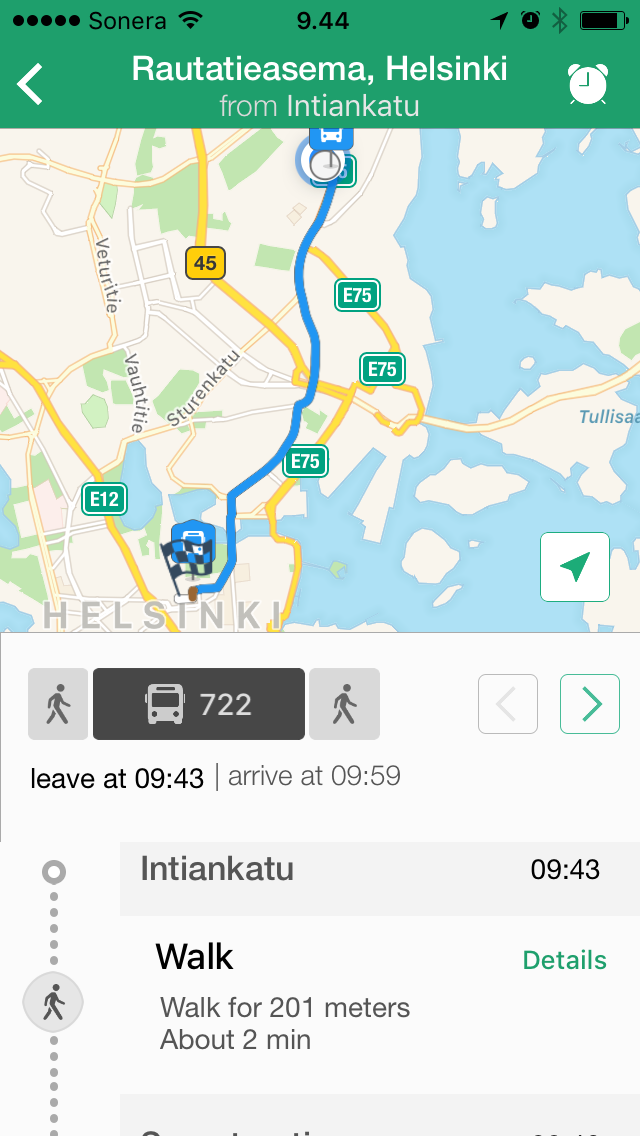
\includegraphics[height=0.6\textwidth]{images/commuter-planning.png}
				\caption{Planning a journey from Kumpula to the Helsinki railway station in Commuter.}
				\label{commuter_planning}
			\end{center}
		\end{figure}
		
		% How this solution uses location awareness? 
		The application relies very much on the location of the user just like any navigation and transportation service. The user's location is visible all the time in the application even if the starting point of a journey differs. Users are continuously shown their surroundings, such as street map, bus stops, stations and service points. While on journey, it is clearly indicated what the upcoming stops are and how long time it takes to reach the desired destination. The transition between lines could never be easier than with this service as is indicates the distance and direction clearly. All in all, this service greatly enhances the location awareness of the user and helps to reach the intermediate and final destinations.
		
		% How does this solution address the challenges? Lack of standards, Positioning, Power consumption, Privacy
		Commuter addresses the challenges as follows. 
	\begin{itemize}
		\item Lack of standards: the service is focused on one mobile platform as it is available only on iOS devices. From the "About" page in the application it is clear that different public APIs are utilized for the accurate data displayed in the application. This means that the timetables of the public transportation and disruptions are loaded from public data sources. These sources are unknown; there is a possibility that they are different format but yet transparent for the user.
		\item Positioning: the positioning works very accurately as an end-user even without internet connection. Seemingly, the position is updated every couple of seconds, which gets a bit more rapid when on journey. This is logical, because users need more updates while using on public transport than when planning their journey.
		\item Power consumption: as an end-user, the application consumes fairly small amount of battery. The service is limited to access data only from a limited number of sensors. For example, it would not benefit from the usage of the camera or microphones and therefore does not use these accessories at all, which saves some battery power.
		\item Privacy: users are not required to enter any log-in credentials nor e-mail addresses in advance of using the applicaiton. This indicates anonymity as an end-user and homogeneity among the user base. If the service provider collects data concerning users, their identity should remain unknown, however their behavior and habits could be interesting to analyze.
	\end{itemize}
	\subsubsection{Tinder}
		% What is this solution briefly? Who is the targeted audience? 
		% How this solution uses location awareness? 
		% How does this solution address the challenges? Lack of standards, Positioning, Power consumption, Privacy
	\begin{itemize}
		\item Lack of standards: 
		\item Positioning:
		\item Power consumption:
		\item Privacy:
	\end{itemize}			
	
	\subsubsection{Sports tracker}
		% What is this solution briefly? Who is the targeted audience? 
		% How this solution uses location awareness? 
		% How does this solution address the challenges? Lack of standards, Positioning, Power consumption, Privacy
	\begin{itemize}
		\item Lack of standards: 
		\item Positioning:
		\item Power consumption:
		\item Privacy:
	\end{itemize}		
		
	\subsubsection{Reslink}
		% What is this solution briefly? Who is the targeted audience?
		Reslink \cite{res16}
		% How this solution uses location awareness? 
		% How does this solution address the challenges? Lack of standards, Positioning, Power consumption, Privacy
	\begin{itemize}
		\item Lack of standards: 
		\item Positioning:
		\item Power consumption:
		\item Privacy:
	\end{itemize}	
		
\section{Privacy}
	
\section{Energy-efficiency}

\pagebreak

\nocite{*}

\bibliographystyle{../tktl}
\bibliography{bibliorgaphy}

\lastpage
\appendices
\pagestyle{empty}
\end{document}


